\chapter{Fundamentação teórica}
\label{chap:Fundamentação teorica}


Para conceituar, fundamentar e dar suporte teórico ao presente trabalho
apresentam-se neste capítulox os tópicos e definições dos segmentos: IoT,
localização contextual de dispositivos e localização baseada em redes sem fio.

\section{Internet das coisas (IoT)}
\label{sec:INTERNET DAS COISAS (IOT)}

Uma das primeiras aplicações e definições de IoT foi feita simultaneamente por Kevin Ashton em
1999 para a \emph{Procter \& Gamble} (P\&G) \cite{ASHTON2009} e
pelo laboratório Auto-ID Labs no Instituto de Tecnologia de
Massachusetts (MIT - \emph{Massachusetts Institute of Technology}) utilizando
identificação por radio-frequência (RFID - \emph{radio-frequency
identification}) \cite{ATZORI2010, Friedemann2011}. Desde então, a IoT cresceu
ultrapassando o escopo da tecnologia RFID, porém sempre com as premissas de ``uma
infraestrutura global para a Sociedade da Informação, habilitando serviços
avançados através da interconexão de coisas (físicas e virtuais) baseadas em
tecnologias, existentes e evolutivas, de informação e comunicação'' descrita por
\apudonline[p.~1, grifo e tradução
nossa]{Wortmann2015}{InternationalTelecommunicationUnion2012}.

Hoje em dia, quase qualquer tecnologia de comunicação acessível a computadores
pode ser utilizada como meio de comunicação entre dispositivos IoT, tornando
o RFID mais uma, porém de grande importância, tecnologia info-comunicacional a
disposição das coisas para sua conexão. Esta gama de tecnologias possibilita uma
variedade equivalente de coisas conectadas. Se a coisa pode usar de uma
tecnologia de conexão, considerando suas restrições de volume, custo e
utilidade, muito provavelmente vai fazê-lo gerando ao menos uma identidade
virtual representando seu objeto físico e seus atributos. Esta identidade
virtual e atributos virtuais serão expostos para todos indivíduos, humanos ou
coisas, que lhe forem convenientes de qualquer lugar do universo virtual,
fazendo efetivamente parte da Internet.

\section{Localização contextual de dispositivos}
\label{sec:Localização contextual de dispositivos}

Em ciência da computação, os termos \emph{"Contexto"} e \emph{"Consciência
de Contexto"} expressam uma ideia recente estudada nos campos de inteligência
artificial e ciência cognitiva desde 1991. O tema "Contexto" ainda é considerado
atual e promissor a ponto de mudar o cenário de negócios nos próximos 10 ano, mas
sem definição simples. Tamanha é a falta de uma definição geral que
realmente funcione para casos reais que existe uma proposta de definir o termo
utilizando uma nova metodologia de pesquisa holística através de mineração e
agrupamento de texto advindo de publicações científicas \cite{Pascalau2013}.

Mesmo sem uma definição permanente em vista, utilizou-se o que é considerado
estado da arte para o termo \emph{"Contexto"} que foi introduzido por
\citeonline{Dey1999} e reforçado por \citeonline{Dey2000}:

\begin{citacao}

	``Contexto é qualquer informação que pode ser utilizada para caracterizar a
	situação de uma entidade. Uma entidade é uma pessoa, lugar ou objeto que é
	considerado relevante para a interação entre um usuário e uma aplicação,
	incluindo o próprio usuário e a aplicação.'' \

	\citeonline[p.~3]{Dey1999} Tradução Nossa.
\end{citacao}

\subsection{Localização contextual}
\label{subsec:Localização contextual}

Das informações contextuais que uma aplicação de cliente móvel pode obter, a
localização é uma das mais importantes. Ajudar pessoas a navegar por mapas,
encontrar objetos e pessoas com os quais tem interesse de interagir é sem dúvida
uma boa meta a ser alcançada com a coleta da localização do cliente
\cite{Bellavista2008}.

Na categoria de Serviços Baseados em Localização (LBS - \emph{Location-Based
Services}) existem duas gerações. A primeira orientada a conteúdo que falhou,
pois a informação de localização era armazenada pela rede (que geralmetne era
administrada por uma empresa de telecomunicações), podendo até ser vendida pelo
provedor a terceiros, causando a sensação de \emph{Spam} (conteúdo não
solicitado) no usuário final ao receber conteúdo desta provedora. Já na segunda
geração, a posse da informação foi movida para o cliente móvel, deixando a cargo
do usuário escolher se ela seria compartilhada e com quem. Esta mudança trouxe
maior engajamento do usuário, resultando numa maior aceitação dessa geração
\cite{Bellavista2008}.


Ao contrário das técnicas atuais, neste trabalho os humanos ou tomadores de
decisão não estarão em posse do cliente móvel, e sim em posse do prédio.
Portanto, a mesma informação, sem degradação em sua importância, passará a ser
coletada e armazenada pelo provedor da rede como nos LBSs de primeira geração.
Esta decisão garante o foco no usuário uma vez que este mudou, antes ele detinha
um cliente móvel, agora ele detem múltiplos. Isso torna a detenção do todo
(coisas dentro do prédio) mais precioso do que o das partes (os clientes móveis)
além da mudança da propriedade da rede para o usuário final, na comparação
celular \emph{versus} \emph{Wi-Fi}.

Uma vez encontrada a localização de um dispositivo, metadados sobre o prédio são
mesclados formando um conjunto rico contextualmente do ponto de vista da
aplicação IoT Prédio como fornecedora principal dos dados para a Internet e,
portanto, seus usuários detentores. Essa riqueza é garantida com metadados sobre
o dispositivo (identificação, nome, histórico, carecterísticas) e sobre o prédio
(ex.: mapa, estrutura de salas, humanos responsáveis e lista de equipamentos) que trazem possibilidades de
extração de informação importantes para os detentores deste prédio e seu
conteúdo. Esta capacidade do prédio deve-se pelo papel de coordenador de
informações e controlador de meta-informações semelhante ao Coordenador em uma
aplicação na arquitetura Modelo-Apresentação-Adaptador-Controlador-Coordenador
(MPACC - \emph{Model-PresentationAdapter-Controller-Coordinator}) proposto por
\citeonline{Roman2001}.


\subsection{Contexto de um dispositivo em um prédio}
\label{subsec:Contexto de um dispositivo em um prédio}

Para metadados agregados à informação de posição pelo prédio defini-se que, para uma aplicação IoT, o
modelo de divulgação tem de conter além da posição do dispositivo informação
sobre este (nome, histórico), informação da estrutura do prédio, ligação entre a estrutura
do prédio e a localização do dispositivo e informação
sobre o estado do prédio.


Este modelo visa prover fácil mineração e reutilização de informações por
terceiros que é medida pela disponibilidade e
relacionamento das informações providas. Essa métrica também será utilizada para
avaliar o projeto.

Este foco em reusabilidade vem da definição de Web Semântica (\emph{Semantic
Web}) e de uma de suas realizadoras, a Ligação de Dados (\emph{Linked Data}),
que sugerem o uso de um formato padrão além de ser acessível e gerenciável pelas
ferramentas de exploração. Desta forma a Web de Dados (\emph{Web of Data}) é
construída opondo uma simples coleção de dados \cite{Bizer2009}.

\section{Localização baseada em redes sem fio}
\label{sec:Localização baseada em redes sem fio}

Um sistema de posicionamento pode ser baseado em técnicas
\emph{n-lateração?} de distâncias adquiridas com a medição de características
eletromagnéticas (ex.: potência de sinal) e dos protocolos (ex.: Tempo de
chegada) que já foram explorados anteriormente \cite{Abusubaih2007,
bahillo2009ieee, Feldmann2003}.

Portanto, os sensores seguem as especificações de \emph{WiFi IEEE 802.11}
\cite{Crow1997} e técnicas definidas para \emph{Bluetooth Low Energy (BLE)}
\cite{Hossain2007} devido a semelhança da área de cobertura (até 100 metros,
geralmente utilizado até 20 metros) e frequência (no caso de 2.4GHz).

Para construir estes sensores uma plataforma de hardware adequada é necessária,
para esta escolheu-se o Raspberry Pi \cite{Vujovic2014, Vujovic2015} que já
foi provado funcional no caso de Localização através \emph{Wi-Fi} por
\citeonline{Ferreira2016} especialmente a sua versão 3 que adiciona a capacidade
de sensor \emph{Wi-Fi} e \emph{Bluetooth} em sua placa principal sem
necessidade de adaptadores externos destacando ainda mais sua escolha
\cite{RPI2016}. Em adição, na construção dos sensores foi testada a plataforma ESP8266 bem como
outras alternativas que demonstraram afinidade com essas características.


\section{Trabalhos correlatos}
\label{Trabalhos correlatos}
Neste subcapítulo, apresentaremos alguns projetos semelhantes em objetivo ao daqui
proposto e que motivaram a construção do sensor resultante deste trabalho.

\subsection{Zebra}
\label{subsec:Zebra}

A Zebra é um empresa estadunidense que fabrica e vende tecnologia de marcação,
rastreamento e impressão por computador. Dentre os seus produtos, estão:
computadores móveis, RFID, software, impressoras, tablets, leitores de códigos
de barras, kiosks interativos, entre outros. Já na área de serviços, a empresa
oferece desde o planejamento até a execução de projetos.

A Zebra realizou um estudo (Global Shopper Study) que indicou que os varejistas
apostaram em recursos online que podem aumentar o envolvimento e fidelidade do
consumidor, além, claro, do volume de vendas. Segundo o mesmo estudo, 51% dos
compradores tem um forte interesse em serviços baseados em localização e
\emph{Wi-Fi} em lojas para cupons \emph{mobile}, mapas de compras e receber
assistência. Além disso, 64% dos compradores dizem que estão dispostos a comprar
mais itens se receberem um serviço melhor e mais atenção dos vendedores,
enquanto mais da metade prefere que os varejistas usem a tecnologia para criar
experiência de compra mais eficiente.

A empresa possui o projeto MPact que é um \emph{indoor location} que unifica
\emph{Wi-Fi} e \emph{Bluetooth}. Ele fornece a localização do consumidor em três
níves: presença, zona e posição. Com estas informações é possível saber sobre o
indíviduo: quem é, onde está, quanto tempo fica em certas áreas e quais
produtos está comprando. Esta tecnologia pode ser implementada independente do
ambiente, através do \emph{Wi-Fi}, ou do microposicionamento através do
\emph{Bluetooth}. Com a união dessas duas plataformas é possível saber o tempo
exato e posição exata de onde alguém está.

Em 2016, a empresa implantou no Shopping Cidade Jardim, em São Paulo, uma rede
LAN/WAN sem fio de alta velocidade, com a tecnologia MPact que proporciona aos
seus clientes acesso gratuito ao \emph{Wi-Fi}, juntamente com uma experiência de
compra mais personalizada. Funciona assim, o consumidor assim que possível
acessa o \emph{Wi-Fi} do shopping que pede o \emph{login} no Facebook ou Google. Assim
que o \emph{login} é feito, o MPact fornece visibilidade instantânea ao operador do
shopping em relação aos locais dos compradores no shopping e habilita os
operadores a enviar saudações pessoais, oferecer ofertas especiais ou fornecer
instruções passo-a-passo para um venda ou promoção específica. Hoje, o Cidade
Jardim conta com 180 lojas numa área de 46.000 metros quadrados.

Segundo Claudio Bessa, diretor de markegin digital do shopping, este tipo de
serviço fornece um excelente experiência para os compradores devido a alta
velocidade do \emph{Wi-Fi} e a cobertura. Além disso, segundo ele, os operadores
e varejistas podem entender melhor o comportamento do consumidores, pois eles
podem saber que parte do corredor ou de uma loja o cliente está, quanto tempo
permanece na frente de uma loja e quais produtos mais vendem. Oferecer este tipo
de serviço é uma maneira de ganhar e manter consumidores, crescer no número de
satisfações e ajudar a monitorar os pontos de venda.

\begin{figure}[htb]
	\caption{\label{fig:projeto}Cidade Jardim }
	\begin{center}
		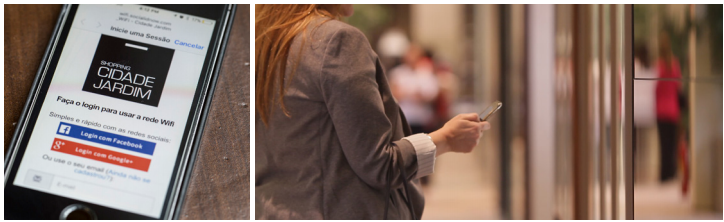
\includegraphics[width=1\textwidth]{020-fundamentacao/img/cidade-jardim.png}
	\end{center}
	\legend{Fonte: Zebra Technologies}
\end{figure}

\subsection{Outras tentativas}
\label{subsec:Outras tentativas}

Outras tentativas bem sucedidas de localizar dispositivos móveis através da rede
\emph{Wi-Fi} são o caso do \emph{Decimeter Level Localization with a Single
Access Point} \cite{Vasisht} e do \emph{Radio Frequency Time-of-flight Distance
Measurement for low-cost Wireless Sensor localization} \cite{Lanzisera2011}.

No primeiro exemplo, uma placa de rede sem fio Intel 5300 com 3 antenas calcula o tempo
de vôo entre uma antena e outra além de utilizar técnicas de mitigação de
multi-caminho, mitigação de identificação de pacote entre outras características
importantes do protocolo \emph{Wi-fi}, como a frequência e sincronização de clientes
para alcançar até 10 centímetros de precisão. Neste caso, as três antenas atuam
como três sensores independentes justa posicionados para executar trilateração.
Esta aplicação é implementada em uma placa instalada em um computador moderno
através do barramento PCI Express com sistema operacional Ubuntu. Ela possui habilidade
de injetar pacotes na rede o que difere muito das arquiteturas embarcadas que
normalmente são encontradas no ambiente de IoT.

O segundo exemplo de aplicação bem sucedida se utiliza de modificações no
hardware de um ponto de acesso do padrão 802.15.4 e alcança precisões de 1 a 3
metros. Este protocolo é mais encontrado em comunicações de longa distância ou
sensíveis a uso de energia que são frequentes em aplicações embarcadas.

\begin{figure}[htb]
	\caption{\label{fig:projeto}Radio Frequency Time-of-Flight Distance Measurement}
	\begin{center}
		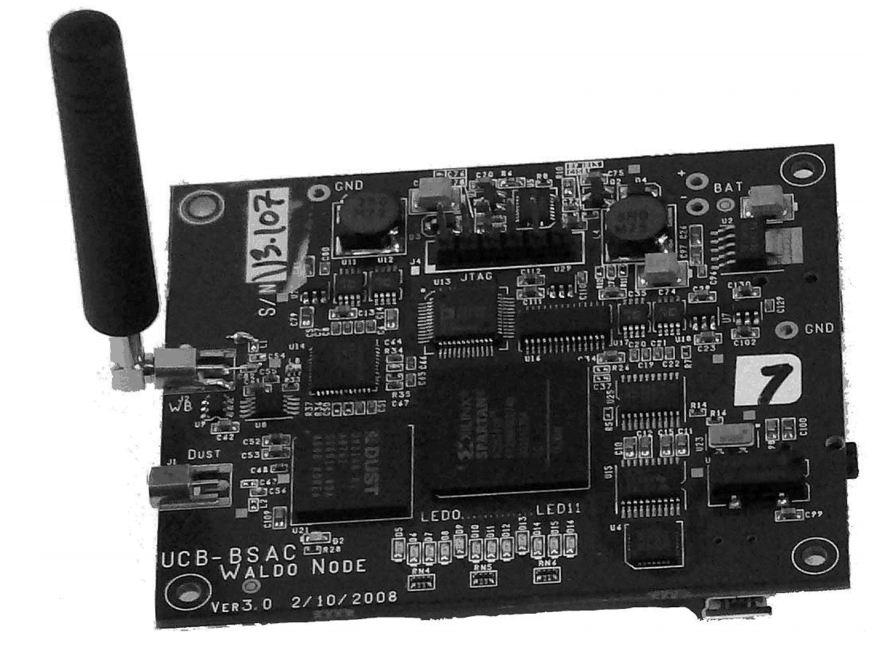
\includegraphics[width=1\textwidth]{020-fundamentacao/img/radio.png}
	\end{center}
	\legend{Fonte: \citeonline{Vasisht}}
\end{figure}
